\documentclass[12pt]{article}

% add some essential packages, some might not be used
%\usepackage{CJKutf8}
\usepackage[T1]{fontenc}
\usepackage[utf8]{inputenc}
\usepackage[usenames,dvipsnames]{color}
\usepackage{authblk}
\usepackage{xeCJK}
\usepackage{ragged2e}
\usepackage{amsmath}
%\usepackage[a4paper,margin=2in,bottom=1.0in]{geometry}
\usepackage{url}
\usepackage{array}
\usepackage{bbding}
\usepackage{amssymb}
\usepackage{graphicx}
\usepackage{adjustbox}
\usepackage{subcaption}
\usepackage{caption}
\usepackage{booktabs}
\usepackage{float}
\usepackage{appendix}
\usepackage{url}
\usepackage[english, russian]{babel}
\usepackage{adjustbox}
\usepackage{textgreek}
\usepackage{NotesTeX}
\usepackage{lipsum}
\usepackage[procnames]{listings}
\usepackage{wasysym}
\usepackage{amsthm}
\usepackage{framed}
\usepackage[procnames]{listings}
\usepackage[scaled=0.9]{DejaVuSansMono}
\usepackage{pythonhighlight}
%\usepackage{marvosym} % coffeecup 

\usepackage[ruled,vlined]{algorithm2e}

\usepackage{rotating} % for the horizontal page table

\usepackage{tikz}
\usetikzlibrary{calc}
\usetikzlibrary{matrix}
\usetikzlibrary{positioning}
\usepackage{color}
\usepackage{setspace}
% python highlight package
\usepackage{pifont} % checkmark package 

\newcommand{\zn}{\mathbb{Z}}
\newcommand{\cn}{\mathbb{C}}
\newcommand{\qn}{\mathbb{Q}}
\newcommand{\rn}{\mathbb{R}}
\newcommand{\pn}{\mathbb{P}}
\newcommand{\fn}{\mathbb{F}}
\newcommand{\nn}{\mathbb{N}}



\usepackage{tcolorbox} % package for making colorful box

 \setlength{\parskip}{0.15cm} % change the paragraph spacing
\renewcommand\labelitemi{$\vcenter{\hbox{\tiny$\bullet$}}$} % set the bullet size as tiny

% \newcommand*\rot{\rotatebox{90}} % for rotate text

%\usepackage{courier}

\newenvironment{fullmodel}{
			\smallskip\noindent
			\begin{minipage}{\textwidth+\marginparwidth+\marginparsep}\smallskip\smallskip}
			{\smallskip\smallskip\end{minipage}\vspace{.1in}
			}



\title{{\Huge 人工智能基础(高中版)}\\{\Large{辅导讲义}}}
\author{王斐 Michael\footnote{\href{https://www.michaelyunfei.com}{\textit{Author Website}}}}

\affiliation{School of Mathematics and Statistics, UCD}
\emailAdd{michael.yunfei@gmail.com}


\numberwithin{equation}{section}
\numberwithin{figure}{section}


\newenvironment{question}[2][Question]{\begin{trivlist}
\item[\hskip \labelsep {\bfseries #1}\hskip \labelsep {\bfseries #2.}]}{\end{trivlist}}


\begin{document}
  \maketitle
  \flushbottom
  \newpage
  \pagestyle{fancynotes}

\definecolor{franceblue}{RGB}{156, 195, 228}
\definecolor{medblue}{RGB}{88, 157, 196}


\setcounter{part}{2}

\part*{第三章:神经网络模型初探}

\marginnote{\begin{tcolorbox}[colframe=gray]《大学》中语:知止而后有定,定而后能静,静而后能安,安而后能虑,虑而后能得。物有本末,事有终始。知所先后,则近道矣。\end{tcolorbox}}

亲爱的同学们,从这一章开始我们将会接触目前比较流行的人工智能模型-神经网络模型。相较前一章节,本章难度有所提升,而且模型背后的相关概念更加抽象。如果你已经开始阅读第三章节的内容,或许你会觉得\textit{`不知所云'}或者\textit{`无从下手'}。 对于任何一个初学者来说,这都是很正常的经历,希望你们不要气馁,更不要怀疑自己。此时此刻,希望同学们仍然要怀着探索的心态去进入这一章节的学习。

我们将会在接下来的三周里沉浸在神经网络模型中,如果同学们紧跟老师的节奏,按照要求完成\textbf{课前预习,课上笔记,及课后练习}这三个环节,我可以向你们保证,三周之后你们(每一位同学)完全可以:
\begin{itemize}
	\item 理解为什么人工智能在神经网络\sn{Neutral Network}出现后具有了广泛得应用价值;
	\item 掌握神经网络的本质所在,并且了解模型背后的思想精髓所在;
	\item 能够用Python透过向量\sn{Vector}和矩阵\sn{Matrix}进行编写20行左右的小程序,从而以此去理解神经网络的模型设计逻辑;
	\item 能够使用Python中人工智能学习平台,如TensorFlow来进行神经网络的训练和调试,从而可以独立自主得对大量的图片数据进行分析。
\end{itemize}

%\marginnote{\begin{tcolorbox}[colframe=gray]jh\end{tcolorbox}}

为了提高沟通速率且帮助同学们养成良好学习节奏\mn{我大学有个德国的同学曾经自恃聪明,声称自己不需要读任何诗歌就可以作诗,我说你来写一首中文诗歌,他也只能相对无言。每个人的大脑都可以是一个储存器,没有输入就不会有输出,所以`自学成才'的前提是自学。不过老师可以负责任的告诉你,自学你需要花更多时间。独孤很可能会败求,切勿舍近求远。},我们以后会将课前预习,课上笔记,及课后练习简称为C1, C2, C3。比如,如果我说\textit{`你需要在下周一之前完成C1',那就意味着你需要根据我在C1中的指示进行课前预习}。下面的表格是后面课程中C1, C2, C3中的包含的内容以及所设定的预订目标。

\begin{table}[H]
	\centering
	\renewcommand{\arraystretch}{1.6}
	\begin{tabular}{|c|c|c|c|}
		\hline
		& C1 & C2 & C3 \\
		\hline 
		主题& 背景资料阅览 & 课堂老师讲解 & 课后习题和编程 \\
		\hline
		内容& 网络文章和视频 & 辅导讲义和课件 & 数学练习和Python练习 \\
		\hline
		时长 & 30分钟-1小时 & 45分钟 & 2-3 小时 \\
		\hline 
		频率 & 一周一次 & 一周三次 & 一周一次 \\
		\hline 
		 & \checkmark & \multicolumn{2}{c|}{只完成C1好比看了一场有关AI的电影} \\
		\cline{2-4}
		收获&  \checkmark & \checkmark & 不作习题C2完全是浪费时间 \\
		\cline{2-4}
		& \checkmark & \checkmark & \checkmark \\
		\hline 
	\end{tabular}
\end{table}


\setcounter{section}{3}
\subsection{课前预习C1}

按照惯例,本次C1依然有两部分组成:
\begin{enumerate}
	\item 读网络文章, 看网络视频;
	\item 根据指示完成小习题,并且准备在课上使用。
\end{enumerate}

\noindent
\textit{第一部分: 神经网络追本溯源}

人们对人工智能的研究热情由来已久,其中神经网络模型的主要研究兴起于上世纪八十年代。众多研究者中,领军人物包括但不限于:Geoffrey Hinton\mn{杰弗里·辛顿},  Yoshua Bengio and Yann LeCun。他们三位因此也被称为人工智能三教父\mn{Godfathers of AI (Godfathers of Deep Learning)}。我们以Geoffrey Hinton的思路为切入点,来理解神经网络的发展过程和之所以蓬勃发展的深层次原因。

观看Geoffrey Hinton的采访视频,注意思考以下几个问题:
\begin{itemize}
	\item 观看前10分钟\mn{注意视频中配有机器自动加注的英文字母和中文翻译,因此存在一定纰漏,但是不影响整体理解.其中03:50处,他讲到`I think around early 1982...’,而不是`伊拉克发生了什么’。这说明机器和人类一样并不完美,`绝对'的物只在意念中存有!}
	\item 是什么触发了Geoffrey Hinton对人工智能的研究,最初的切入点是什么?
	\item Geoffrey Hinton 比较了英国和美国的学术环境,你从中有什么启发?
	\item Geoffrey Hinton 提到了心理学界和AI领域对\textit{知识}的理解,何谓知识?
	\item 视频连接:\url{https://www.bilibili.com/video/av69581590/}
\end{itemize}

\definecolor{steelteal}{RGB}{95, 124, 138}

\begin{fullmodel}
	\begin{tcolorbox}[title={哲学延伸},fonttitle=\large,colframe=medblue]
		   认识论是哲学研究范畴中比较重要的一枝,视频中Geoffrey提到`how concepts are relate to other concepts' (一个概念与其它概念的联系),这是目前有关知识的普遍共识。比如描述一朵花,需要高度,大小,颜色,等等一系列的概念堆积。而这些概念的关联就构成了我们的知识。\textbf{后面我们介绍深度学习模型时,你会接触到`卷积'和`池化'等概念}。这些新鲜的名字背后本质上是通过一个个数学模型来模拟概念关联和堆积,从而进行智能判断。深度神经学习本质上是对人的\textbf{生物仿生模拟},我们在调试模型时需要反向调整参数,这与我们实际生活中的学习如出一辙。比如,你第一次接触滚烫的热水时,会感到疼痛,接受到该信号后,下一次你会\textbf{试探性}得调整动作去接触热水,这就是人类反向调整的过程。
		   
		\setlength{\parindent}{5ex}
		Geoffrey能够想出神经学习模型除了与他自己兴趣广泛,对该问题长期关注之外,还与其在英国接受的教育传统有关。认识论的鼻祖可以追溯到笛卡尔(也就是发明XY坐标的那个法国人),但是第一次系统提出`所有的知识都是关联’的是英国哲学家休谟,休谟又启发了德国的大哲学家康德。人类历史上几次\textbf{颠覆}性的概念,如牛顿万有引力,达尔文进化论,休谟的认识论,亚当斯密的市场经济理论,图灵的计算边界论等都首先出自英国,是因为长期以来英国教育注重热爱自然,着重培养学生仔细观察记录和思考有关。同学们正值青春年华,不要泯灭了对自然和生命得热爱。以后人工智能可以帮助人类去完成更多机械化的任务,那么想象力就变得更加重要。
	\end{tcolorbox}
\end{fullmodel}

观看华为总裁任正非的采访视频,注意思考以下几个问题:
\begin{itemize}
	\item 观看视频中10:00 - 15:00分钟段
	\item 为什么任正非说人工智能是`计算机+统计学'?
	\item 为什么有一种论调称`数据就是未来的石油’?
	\item 视频连接:\url{https://m.sohu.com/a/290453977_652527/}
\end{itemize}

\begin{fullmodel}
	\begin{tcolorbox}[title={打破人工智能的迷思},fonttitle=\large,colframe=medblue]
		一段时间以来,有关人工智能,大数据的话题占据了很多网络报刊的头条位置,也使得我们的生活有所喧嚣,很多人也是人云亦云般得吹泡泡。在从大得方向上掌握了,深度神经网络学习模型实际上是对人的生物仿生模拟之后,我们会通过本章的学习,解答以上两个问题。简单讲,一个人的成长需要千锤百炼,人工智能也需要学习,不过人类是通过眼耳鼻喉舌五官来进行感觉输入和经验收集,最终进行意识加工和输出,然而电脑喝得是数据,吐出来的是`牛奶'.有朝一日,人工智能很有可能会`横眉冷对千夫指,俯首甘为孺子牛'。让我们共同期待吧! 
	\end{tcolorbox}
\end{fullmodel}


\noindent
\textit{第二部分: 课前小习题\mn{勿以善小而不为:比如现在火爆的5G网络,归根结底起源于是对一个多项式的求解。5G是错误纠正码的一种(error correction code),而错误纠正码中传输速率最大的一种模型依靠的是伽罗瓦理论(Galois theory),而这位法国的年轻人提出这个理论最初是解决下面这个问题: 取任意$a, b, c, d, e,f \in \rn$(实数$\rn$包括有理数和无理数),下面五项式方程是否有解, \begin{align*}
	ax^5 + bx^4+cx^3 + dx^2 + ex + f = 0
\end{align*}同学们肯定都知道如何解决二项式$ax^2+bx+c=0$是否有解,有兴趣也可以把解决四项式或者五项式作为爱好培养。Galois只是感兴趣而研究这个问题,但是该问题所引发的一般理论成为了现代代数的的核心,广泛应用信息传输中。Galois为博取一女生的欢心,在与情敌的决斗中受重伤,于英年20岁时卒。法国政府将其名字刻在Eiffel Tower上,以表尊缅。}}

课前小习题是为了帮助同学们熟悉机器的思考方式,并且能够理解背后的数学算法。简而言之,机器或者电脑的思考方式就是`一步一脚印'的方式,也就是\textit{具体问题机械分解化,机械分解数学化,数学运算代数化,代数问题向量/矩阵化}。这些小习题都非常简单,但是`法力无边'。

\begin{question}{C1-Q1}
	计算机又被称为电脑,电脑的核心是芯片,芯片的计算单元是晶体管。晶体管通电可以表示一种状态,称之为1,晶体管断电可以表示一种状态,称之为0。假设我们有下列三个并排晶体管,每个晶体管中可以填0或者1。\textit{问三个晶体管中至多可以存放多少个信息}(只要数字不同就可以被成为信息,比如0跟101不同,那么这两个可以算两个信息。1和1只能算作一个信息)?
	\begin{figure}[H]
		\centering
		\begin{tikzpicture}
		\draw[step=1cm,gray,thin] (0,2) grid (3,1);
	\end{tikzpicture}
	\end{figure}
\end{question}

\begin{question}{C1-Q2}
	将所有可能的信息(实际上就是由0和1组成的序列)按照你认为\textit{符合逻辑}的方式进行排列,比如 $0, 1, 00, 01, \cdots$ 或者 $010, 000, 01, 00,\cdots$. 
\end{question}


\begin{question}{C1-Q3}
	可能同学们在第一小问中很快就可以得出答案,共计有$2^3=8$个信息单元,但是如果你把所有的可能都写出后,你会发现答案是$2+2^2+2^3=14$.
\end{question}

\begin{remark}
如果我告诉你以下数字的二进制表达,你能否根据以上习题反向推出二进制的设计机制?
\end{remark}
\begin{table}[H]
	\centering
	\renewcommand{\arraystretch}{1.5}
	\begin{tabular}{cc}
	\hline 
		十进制数字 & 二进制数字 \\
		\hline 
		14 & 1110\\
		13 & 1101 \\
		12 & 1100 \\
		11 & 1011 \\
		\hline 
	\end{tabular}
\end{table}	

\begin{question}{C1-Q4}
	(排列组合题)现在有以下7个空位,如果有三个捆绑在一起的信息$ABC$(排序不可改变),且每个字母占位一个空格,请问至多有几种方式将$ABC$放到下面的方格中去?
		\begin{figure}[H]
		\centering
		\begin{tikzpicture}
		\draw[step=1cm,gray,thin] (0,2) grid (7,1);
	\end{tikzpicture}
	\end{figure}
\end{question}

\begin{question}{C1-Q4}
(排列组合题)现在有以下一个$2\times 2$ 和一个$5\times 5$的矩阵, 其中$2\times 2$ 的矩阵中已经被填充了$A,B,C,D$(如图所示),请问按照现有$A,B, C, D$的排列方式,在$5 \times 5$的矩阵中,至多有多少种填充方式?
		\begin{figure}[H]
		\centering
		\begin{subfigure}[b]{0.45\textwidth}
			\centering
		\begin{tikzpicture}
		\draw[step=1cm,gray,thin] (0,0) grid (2,2);
		\draw (0.5, 1.5) node{A};
		\draw (1.5, 1.5) node{B};
		\draw (0.5, 0.5) node{C};
		\draw (1.5, 0.5) node{D};
	\end{tikzpicture}
		\end{subfigure}
		\begin{subfigure}[b]{0.45\textwidth}
			\centering
		\begin{tikzpicture}
		\draw[step=1cm,gray,thin] (0,0) grid (5,5);
	\end{tikzpicture}
		\end{subfigure}
	\end{figure}	
\end{question}


\begin{question}{C1-Q5}
	(颜色填充)下图左边的坐标中定位了红,绿,蓝三个点和一个橙色点\mn{如果同学有颜色识别困难的,可以问下父母或者身边的朋友。},如果我们将矩阵的纵列(row)代表坐标的$x$轴,将矩阵的横列(columns)代表$y$轴,根据所在的坐标将这三个点定位到右边的矩阵去中。我们使用数字代码1代表红色,2代表绿色,3代表蓝色。
	\begin{figure}[H]
		\centering
		\begin{subfigure}[b]{0.45\textwidth}
			\centering
			\begin{tikzpicture}[domain=0:2]
				\draw[thick,color=gray,step=.5cm, dashed] (-0.5,-.5) grid (3,3); \draw[->] (-1,0) -- (3.5,0) node[below right] {$x$}; \draw[->] (0,-1) -- (0,3.5) node[left] {$y$};
				\draw (-0.2, -0.2) node{0};
				\draw (-0.2, 1) node{2};
				\draw (-0.2, 2) node{4};
				\draw (2, -0.2) node{4};
				\draw (1, -0.2) node{2};
				\node at (1,1.5) [circle,draw=blue!50,fill=blue] {};
				\node at (2,2) [circle,draw=red!50,fill=red] {};
				\node at (3,1) [circle,draw=green!50,fill=green] {};
				\node at (2,0.5) [circle,draw=blue!50,fill=orange] {};
			\end{tikzpicture}
		\end{subfigure}
		\begin{subfigure}[b]{0.45\textwidth}
			\centering
			\begin{table}[H]
			\centering
			\renewcommand{\arraystretch}{1.3}
				\begin{tabular}{c|c|c|c|c|c|}
					& y1 & y2 & y3 & y4 & y5 \\
					\hline 
					x1 &  &  & & &  \\
					\hline 
					x2 &  & &3 & &  \\
					\hline 
					x3 &  &  & & &  \\
					\hline 
					x4 &  &  & &1 &  \\
					\hline 
					x5 &  & 2 & & &  \\
					\hline 
					x6 &  &  & & &  \\
					\hline 
				\end{tabular}
			\end{table}
		\end{subfigure}
	\end{figure}
	因为除红、绿、蓝三色之外的颜色都可以由这三个颜色来调和,因此图中橙色点可以用$1, 2, 3$的组合来代表。\mn{因为颜色还有浓艳的问题,所以标准的红、绿、蓝,也就是速成的RGB颜色代码是用255来表示浓度均值的。比如红色的代码是(255, 0, 0),绿色为(0, 255, 0), 蓝色为(0, 0, 255)。比如老师个人很喜欢的\colorbox{franceblue}{法式浅蓝色}的代码是(70, 136, 241)。}
\end{question}


\begin{question}{C1-Q6}
	(简单向量计算)请根据提示完成下列向量和矩阵的计算:
	\begin{align*}
		\begin{bmatrix}
			1 \\
			2 \\
			3 \\
		\end{bmatrix} + \begin{bmatrix}
			2 \\
			6 \\
			9
		\end{bmatrix} = \begin{bmatrix}
			3 \\
			8 \\
			 \\
		\end{bmatrix}; & &  \begin{bmatrix}
			1 & 3 \\
			5 & 6 
		\end{bmatrix} + \begin{bmatrix}
			2 & 7 \\
			6  & 8 
		\end{bmatrix} = \begin{bmatrix}
			3 & \\
			11 & 14 
		\end{bmatrix}
	\end{align*}
\end{question}


\begin{question}{C1-Q7}
	(Python编程题) 阅读下列代码,并且复制到你自己的Python平台上运行且查看结果。以下代码是我们C1-Q1到C1-Q6,问题所涉及概念的程序演练\mn{Numpy 是Python中常用的数据处理扩展程序,其全称为 Numberical Python (数值计算的Python)。需要提醒同学们的是。Python语言的发展是一个不断融合其它编程语言的过程。其中,对其影响最大的几个有: C, C++, Java; Matlab; R. 其中第一类主要是对Python的性能的语言结构上的影响。第二类Matlab是对其数值计算和可视化的影响(你甚至可以说,Numpy+Matlplot = Matlab)。比如向量的建立在Matlab中可以直接输入[1, 2, 3],Python的输入仿照了Matlab,再比如np.zeros([3, 3])就是直接复制Matlab。另外,Python中常用的可视化工具Matplotlib,全称是Matlab Plot Library,名字就不言而喻了。因为R语言在统计和数据处理上有广泛得应用,所以Python的pandas这个扩展程序主要是借用了R语言中dataframe这个概念。}。
\end{question}

\begin{python}
# Chapter 3 Pre-lecture Exercise
# 第三章课前练习
# @ Michael

# Import essential packages
# 导入必要扩展

import numpy as np

# Create a vector and matrix,创建向量和矩阵

a = np.array([1, 2, 3])
print(a)
type(a)
a.dtype
a.ndim
a.shape

a1 = np.array([4, 5, 6])
a2 = np.array([7, 8, 9])
print(a1+a2)  # 简单的矢量计算

b = np.array([1, 2, 3], [5.6, 7.8, 9.9])  # 错误的输入
b = np.array([[1, 2, 3], [5.6, 7.8, 9.9]])
b.dtype
b.ndim
b.shape  # always use shape to check the dimension
print(b)

b1 = np.array([[1, 2, 3], [4, 5, 6], [7, 8, 9]])
b2 = np.array([[9, 8, 7], [6, 5, 4], [3, 2, 1]])
b1.shape
b2.shape
print(b1+b2)

np.ones([3, 3])  # 快速创建3x3的0矩阵
np.zeros([6, 6])  # 快速创建6x6的1矩阵
\end{python}
\noindent
\textcolor{blue}{C1-Q1的程序化解决}\mn{Python的主要对象单元有:int, float, str, tuple, list, range, dict. 其中后四个是具有一定结构的数据单元,很多更高层级的程式和扩展都是依托在这四个结构数据单元上建立的。比如我们使用的Numpy,很多指令是依托在list上,即[ ],所以你在使用numpy的时候,数据的输入都要加上中括号。有关Python的语言结构和特性我们会再具体的应用时,酌情进行讲解。}
\begin{python}
# C1-Q1 的程序化解决

def comper(n, q):
    # A function for calculating all possible combinations of sequences
    # Input:
    # n - maximial length of sequence
    # q - number of digits, e.g., 2 means binary, 3 means ternary
    # Output: number of all possible sequences we can get given n and q
    # 计算所有可能数组
    # 输入:
    # n - 数组的长度的最大值
    # q - 可选数值,比如2 意味着二进制可选0, 1; 3意味着可选0, 1, 2
    # 输出: 所有可能数组的数量
    t = 0  # initialize a variable to store the result
    # 初始化一个变量t,用来储存结果
    for i in range(n):
        temp = pow(q, i+1)
        t = t + temp
    return(t)


# Test our function, 测试我们的方程
result = comper(3, 2)
print(result)
# Try different parameters
comper(32, 2)  # 8589934590
comper(64, 2)  # 36893488147419103230
comper(32, 4)  # 24595658764946068820
comper(64, 4)  # 453709822561251284617832809909024281940

# HOPE, now you understand why we need quantum computer
# 希望现在你能够理解为什么我们需要量子计算器了	
\end{python}

\noindent
\textcolor{blue}{C1-Q5的Python作图}。\mn{就像我们在C1-Q5中手动作图一样,Python在作图时也需要你给出X—Y上的点。计算机作图和数据可视化已经可以成为单独的一门学科,数据可视化比较常用的编程语言是Javascript,比如D3.js和Chart.js。你在网络上看到的很多的数据动画都是使用以上两种语言制作的。此外,R语言的数据可视化也比较流行,Python正在奋起直追,比如最新的Python作图拓展Seaborn。\begin{figure}[H]
	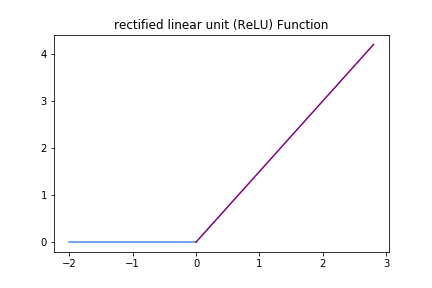
\includegraphics[width=0.4\textwidth]{fig/relu}
\end{figure}\begin{figure}[H]
	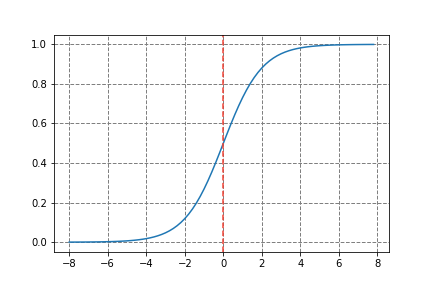
\includegraphics[width=0.4\textwidth]{fig/sigmoid}
\end{figure}}
\begin{python}
# Chapter 3 Pre-lecture Exercise
# 第三章课前练习
# @ Michael

# Import essential packages
# 导入必要扩展

import numpy as np
import matplotlib.pyplot as plt

# Play with colours in Python
# 简单的颜色绘图
# We will use matplotlib to plot a very simple function 
# with varied colours
# 我们将会使用 matplotlib 绘制简单的方程图形并且调试不同颜色

plt.plot([2], [3], 'bo')
plt.plot([4], [4], 'ro')
plt.plot([5], [2], 'go')
plt.axis([0, 6, 0, 7])  # change the range of axis
plt.grid(color='gray', linestyle='--', linewidth=1)  # add grid
plt.title('My first plot')


# plot ReLU function
x1 = np.arange(-2, 0.2, 0.2)
x2 = np.arange(0, 3, 0.2)
plt.plot(x1, 0*x1, color=(70/255, 136/255, 241/255))
# RGB(70, 136, 241)
plt.plot(x2, 1.5*x2, 'purple')
plt.title('rectified linear unit (ReLU) Function')


# plot sigmoid function
x3 = np.arange(-8, 8, 0.2)
y3 = np.exp(x3)/(1+np.exp(x3))
plt.plot(x3, y3)
plt.grid(color='gray', linestyle='--', linewidth=1)  # add grid
plt.axvline(x=0, color=(243/255, 66/255, 53/255), linestyle='--')
# add vertial line
\end{python}
\noindent
\textcolor{blue}{三色图结构}:
下面Python编程是对图片的数字化解构,这一部分程序的运行我们在\textbf{编程练习课中会进一步讲解},因此预习该部分时,稍微浏览即可,无需深入探究。另外,课堂中我们还会进一步探究图片的存储结构和颜色结构,所以请`稍安勿躁'。\mn{计算机图形学已经成为一门独立的学科,而且是一个很庞大的产业。比如苹果的创始人之一Steve Jobs(乔布斯)最初设立苹果公司的初衷就是想要一款可以显示精美字体的计算机,而不是他认为很`丑陋’的windows。如果经常浏览国外网站的同学可能会注意在网页审美设计上,我们还有很大的进步空间。比如浙大的官网,就让人觉得该校的网页设计专业可能不会太好,否则设计的网站不会如此的让人怀疑自己是否具有`信息密集恐怖症'。\textbf{特别提醒}:我们在Python环境下进行图片处理时,优选jpg格式,尽量避免使用png格式。具体的原因和不同情况下的转换,我们会进一步讲解。不过如此的传统也有好处,就是你会发现中国很多的网页设计都像是`头条’设计,一个方框内放一排排的文字再陪一张图片(喝一瓶娃哈哈,解解渴吧)。}
\begin{python}
# Chapter 3 Pre-lecture Exercise
# 第三章课前练习
# @ Michael

# Import essential packages
# 导入必要扩展

import numpy as np
import matplotlib.pyplot as plt
import matplotlib.image as mtmg

# Discover images (探索图片)
# We will import two images and explore how computer store and display images
# 我们将会读取两张图片来探索计算机是如何存储和显示图片的

# The cute panda 可爱的大熊猫
im_panda = mtmg.imread(
    '/Users/Michael/Documents/MDLforBeginners/Chapter3/Code/Images/panda.JPG')
# read panda image 熊猫图片读取
plt.imshow(im_panda)  # show image, 图片显示

im_panda.shape  # (1400, 1400, 3)
print(type(im_panda))   # <class 'numpy.ndarray'>
print(im_panda[:10, :10, 1])  # print 10 by 10 matrix in the second layer
plt.imshow(im_panda[:, :, 0], cmap='gray')
plt.imshow(im_panda[:, :, 1])
plt.imshow(im_panda[:, :, 2])
print(im_panda[700:710, 700:710, 0])
print(im_panda[700:710, 700:710, 1])
print(im_panda[700:710, 700:710, 2])

fig, ax = plt.subplots(nrows=1, ncols=3, figsize=(15, 9))
for i, ax in zip(range(3), ax):
    split_temp = np.zeros(im_panda.shape, dtype='uint8')
    split_temp[:, :, i] = im_panda[:, :, i]
    ax.imshow(split_temp)


# The Mosaic Painting 马赛克绘画
# prefer jpg format, rather than png format
im_mosaic1 = mtmg.imread(
    '/Users/Michael/Documents/MDLforBeginners/Chapter3/Code/Images/Mosaic1.jpg')
plt.imshow(im_mosaic1)
im_mosaic1.shape  # (1034, 1562, 4)
print(im_mosaic1[:10, :10, 1])
plt.imshow(im_mosaic1[:, :, 0])
print(im_mosaic1[700:710, 700:710, 0])
print(im_mosaic1[700:710, 700:710, 1])
print(im_mosaic1[700:710, 700:710, 2])

fig, ax = plt.subplots(1, 3, figsize=(15, 9))
for i, ax in zip(range(3), ax):
    split_temp = np.zeros(im_mosaic1.shape, dtype='uint8')
    split_temp[:, :, i] = im_mosaic1[:, :, i]
    ax.imshow(split_temp)


# The RGB Mosaic
# 三色马赛克
im_rgbmosaic = mtmg.imread(
    '/Users/Michael/Documents/MDLforBeginners/Chapter3/Code/Images/rgbmosaic.jpg')
plt.imshow(im_rgbmosaic)
im_rgbmosaic.shape

# pin down the red color
print(im_rgbmosaic[500:520, 600:620, 0])
print(im_rgbmosaic[500:520, 600:620, 1])
print(im_rgbmosaic[500:520, 600:620, 2])
plt.imshow(im_rgbmosaic[500:520, 600:620, :])

# pin down the blue color
print(im_rgbmosaic[500:520, 230:250, 0])
print(im_rgbmosaic[500:520, 230:250, 1])
print(im_rgbmosaic[500:520, 230:250, 2])
plt.imshow(im_rgbmosaic[500:520, 230:250, :])

# pin down the green color
print(im_rgbmosaic[800:820, 830:850, 0])
print(im_rgbmosaic[800:820, 830:850, 1])
print(im_rgbmosaic[800:820, 830:850, 2])
plt.imshow(im_rgbmosaic[800:820, 830:850, :])	
\end{python}
\noindent
\textcolor{purple}{反馈统计}:请扫描右边二维码,回答对此次课前预习的评估,只有三个问题。Michael 表示非常感谢,请同学多多配合。老师会根据你们的反馈对下一次C1进行提升和改进。填问卷的时候记得喝一杯茶或者咖啡$\heartsuit$。 \begin{marginfigure}
	\centering
	
\includegraphics[width=\textwidth]{fig/C3C1qrcode}
\end{marginfigure}


\newpage
\subsection{课堂讲义C2}

从这一小章节\mn{课堂讲义里的内容是你应该重点学习的内容,学期末的考核所包含的知识点,都涵盖在课堂讲义中,所以你要做到`熟读百遍,而有备无患'。}开始,我们开始进一步学习神经网络模型。按时完成C1的同学,或许已经对人工智能的广泛应用和蓬勃发展已经有了一定的了解。那么接下来,我们就开始系统学习或者说系统训练你们的`人工智能’思维。\textbf{因为这是高中课程,所以我的授课重点是训练你用人工智能解决问题的思维方式}, 在此基础上教授你相应的编程工具。本章节的学习重点有:
\begin{itemize}
	\item 何谓一般的`学习过程’
	\item 传统的问题解决方式和人工智能的解决方式有什么不同
	\item 大数据对人工智能的意涵是什么
	\item 标准神经网络学习模型的组成结构
\end{itemize}

\subsubsection{学习过程的一般性原理}

\begin{fullmodel}
	我们在C1的哲学延伸中(p.2)给出了一个简单的学习过程,即你第一次感受到烫伤后的行为调整过程。同学们可以回忆下自己第一次学自行车,或者第一次使用手机等学习过程中,都包括以下三个基本过程:
	\begin{itemize}
		\item 认知对象(问题)的接触,认知感觉和经验的揽集;
		\item 调用已有概念或知识对所在的场景进行分析;
		\item 做出判断和行动指令,并且有所行动。\begin{itemize}
		\item 如果所做判断和行动,符合预期目标,则维持;
		\item 否则进行修正和调整
		\end{itemize}
	\end{itemize}
	
对以上的学习和认知过程,我们简单概况为一个认知框架:
\begin{figure}[H]
	\centering
	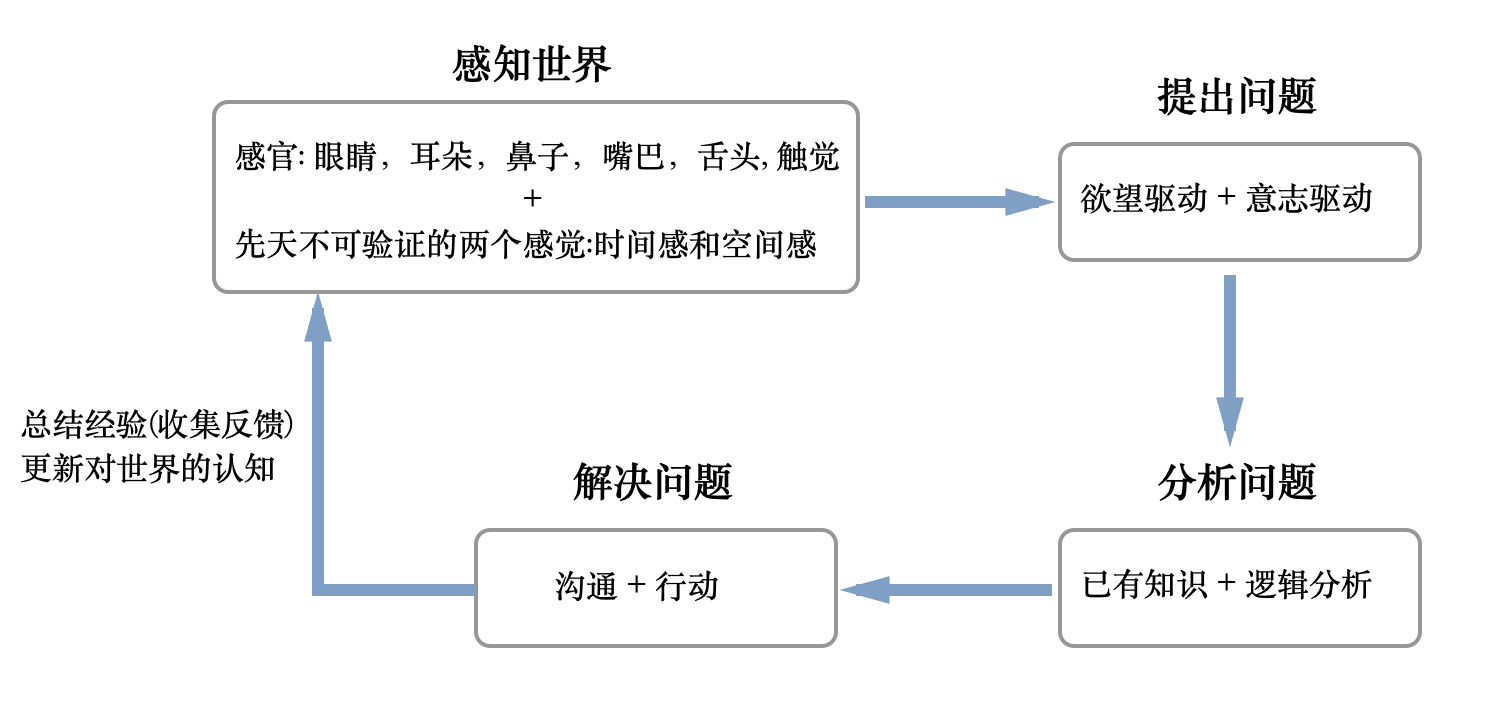
\includegraphics[width=0.69\textwidth]{fig/epismeflow}
\end{figure}

传统的问题解决方法和人工智能解决方法都符合以上框架,但是两者在对具体问题的解决上\textbf{有很大的不同}!
\end{fullmodel}

\subsubsection{传统问题解决方式 VS. 人工智能问题解决方式}

传统的问题解决方式和人工智能问题解决方式最大的不同体现在以下两个方面:
	\begin{itemize}
		\item 传统的问题解决方式着重对问题进行分步骤拆解和处理;
		\item 人工智能对问题的解决方式着重对整个流程的两个端口进行数据和模型联通。
	\end{itemize}
我们通过具体的三个个案例来进行详细的分析,案例一是有关商业广告的投放,案例二是有关信用卡违约,案例三是谷歌AlphaGo(阿尔法狗)的`blackbox'(黑箱)模式。

\definecolor{deepramp}{RGB}{104, 25, 65}

\noindent
\textcolor{deepramp}{案例一} 商业广告投放: 传统的商业广告投放在确定了目标客户后,会通过各种方式(比如问卷调查,消费行为习惯,心里图谱鉴定)对客户群体通过一些列数据来描述。根据所收集的数据建立相应的模型。这些模型的建立往往经由专业人士,比如管理学毕业的学生,或者经济学毕业的学生来完成。决策者在收集数据和模型建立后,然后进行广告的投放。然而,人工智能下的问题解决框架仍然需要收集大量数据,不过由于数字经济方兴未艾,所以数据的收集变得更加容易。收集数据后,对于广告投放的模型构建上,就不需要太多得研究,因为我们可以选择深度学习模型(deepmind model)让计算机自己去学习。\textbf{机器具体如何学习,是我们本章节的重点内容}。

\hfil

\noindent
\textcolor{deepramp}{案例二} 信用卡违约:传统信用卡违约的解决,同样需要进行数据收集,然后银行会聘用专业的风险分析师或者精算师,来进行模型的构建。这些模型的构建往往需要概率论和统计学的系统训练。比如精算师会根据不同场景进行风险的计算,然后指导银行进行信用卡的管理。人工智能是在收集大量数据的基础上,对于相关模型进行训练,然后指导银行进行信用卡管理。我们会在课上,进一步讲解机器是如何学习的。

\hfil

\noindent
\textcolor{deepramp}{案例三} AlphaGo: 2016年阿尔法狗战胜之后,科学美国人杂志(Scientific American)采访AlphaGo的设计人员,邀请他们介绍DeepMind(深度神经网络)为什么能够打败人类顶尖棋手。设计人员可以接受他们模型的构造原理,但是具体这个模型内部的运行过程,他们经常戏称为`黑箱作业'(Black Box)。我们会在本节课中解释他们所称的黑箱是何物。科学美国人原文链接:\url{https://www.scientificamerican.com/article/demystifying-the-black-box-that-is-ai/}


\subsubsection{神经网络模型机制}

\begin{fullmodel}
	教材中有两张图片,即图3-15和图3-19,给出了神经网络模型的工作流程。我们把两个图片中的模型进行简化,绘制下面这张流程图(来源:斯坦福大学深度学习官网)。
\begin{figure}[H]
	\centering
	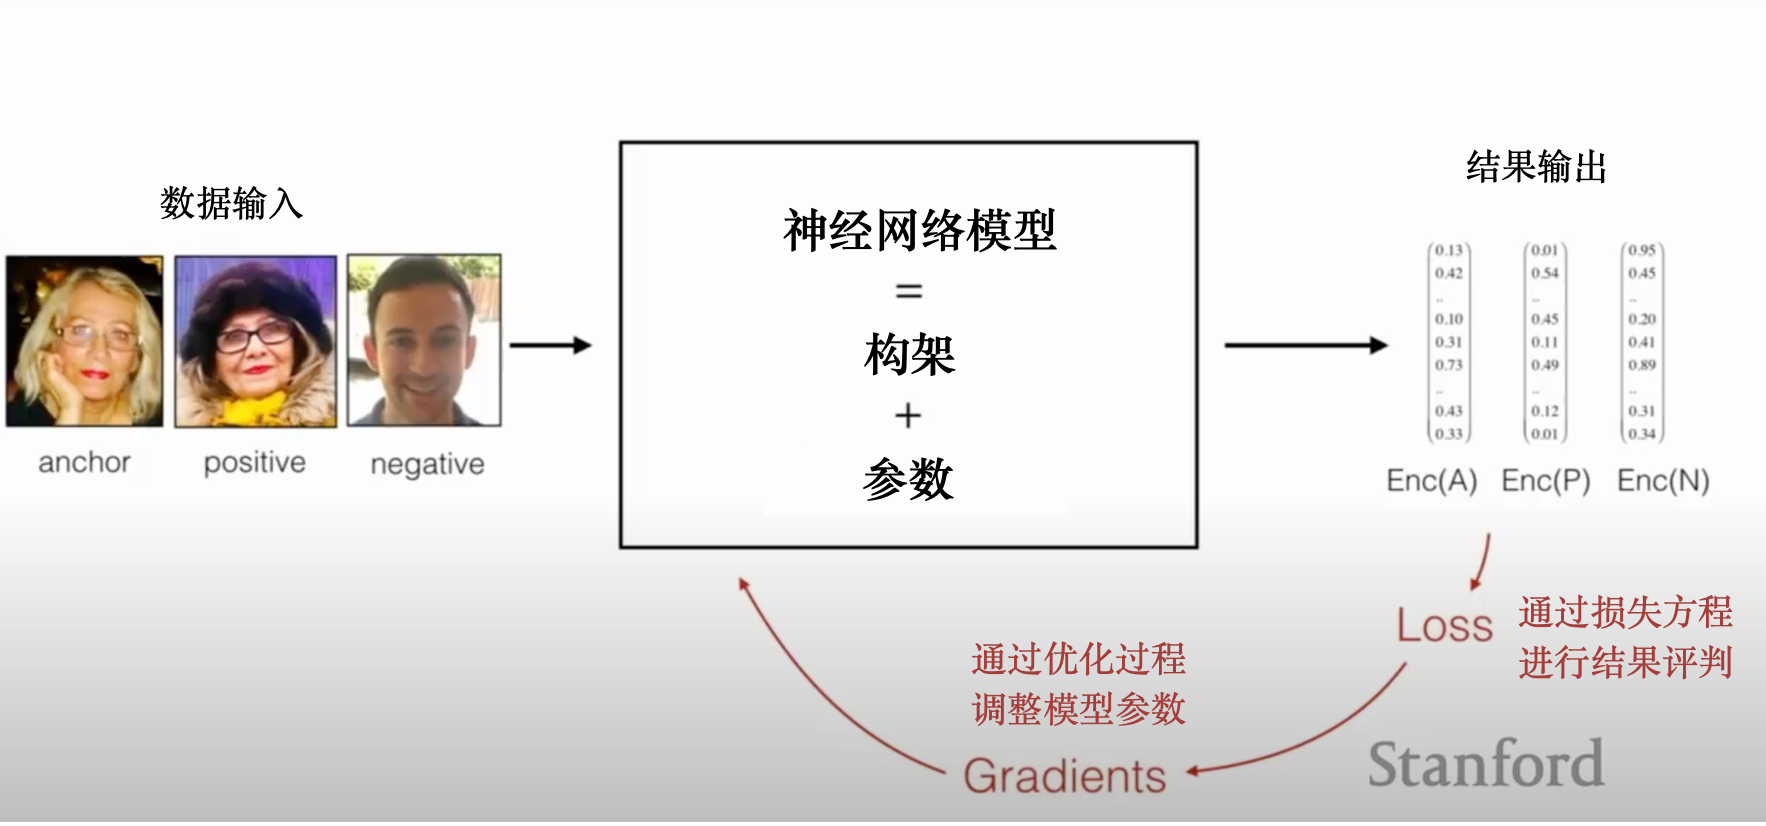
\includegraphics[width=0.8\textwidth]{fig/deepmindflow}
	\caption{深度学习简要框架}
\end{figure}
深度模型的构建的基本单元是一连串的函数组合,这些函数的线性组合构成了我们所称的`神经网络'以及卷积(convolution)的过程。了解这些函数的作用以及卷积的过程对于理解深度学习网络至关重要。所以我们会花费比较多的时间来讲解这些数学概念。
\end{fullmodel}

\subsubsection{数据结构}

因为机器学习和人工智能需要大量的数据,所以非常有必要对数据结构进行定义和分类\mn{生活中最常见的数据形式应该是Excel表格。}。

\begin{definition}
	我们把由数字和对其的描述(有其根据)组成的信息形态,称为\textit{数据};我们将统一在一个描述下的数列,称为\text{数据集}; 有多个数据集构成的一系列数据,称为\textit{数据阵}。
\end{definition}
\begin{marginfigure}
	\centering
	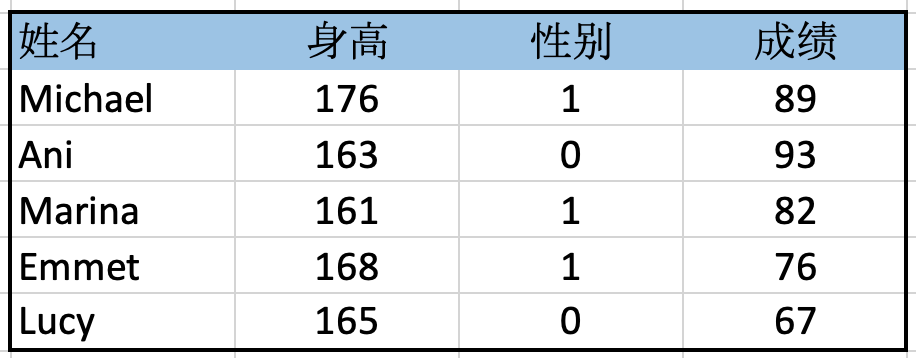
\includegraphics[width=0.9\textwidth]{fig/dataframeEx}
\end{marginfigure}
\begin{remark}
很显然,如果我只给你一个数,比如6, 我们不能称其为数据,因为其缺乏对其的描述。比如,`年方二八’, 年龄16岁,则可以成为数据。	再比如,2019 不是数据,2019年则是数据。
\end{remark}

\begin{example}
数据: 红色-255; 数据集: 颜色: 红255, 绿666, 蓝521; 数据阵:[[颜色:190, 321, 589]; [年份:2019, 2020, 2056]]。右边的表格就是一个数据阵。数据阵(dataframe)是Python和R语言中常用的数据形式。
\end{example}

\begin{definition}
	我们把语言文本,网页信息,图片和影音等的复合数据,称为\textit{多媒体数据集}。
\end{definition}

\begin{example}
下面这张图片是由 Peggy Collins 创作的马赛克数字图画。这张图片在计算机中的存储形式是具有维度$(1400, 1400, 3)$的数据集构成。其中3,是代表的RGB(红绿蓝)三层底色层,每一个色素层是由一个$1400 \times 1400$的矩阵组成。
\begin{figure}[H]
	\centering
	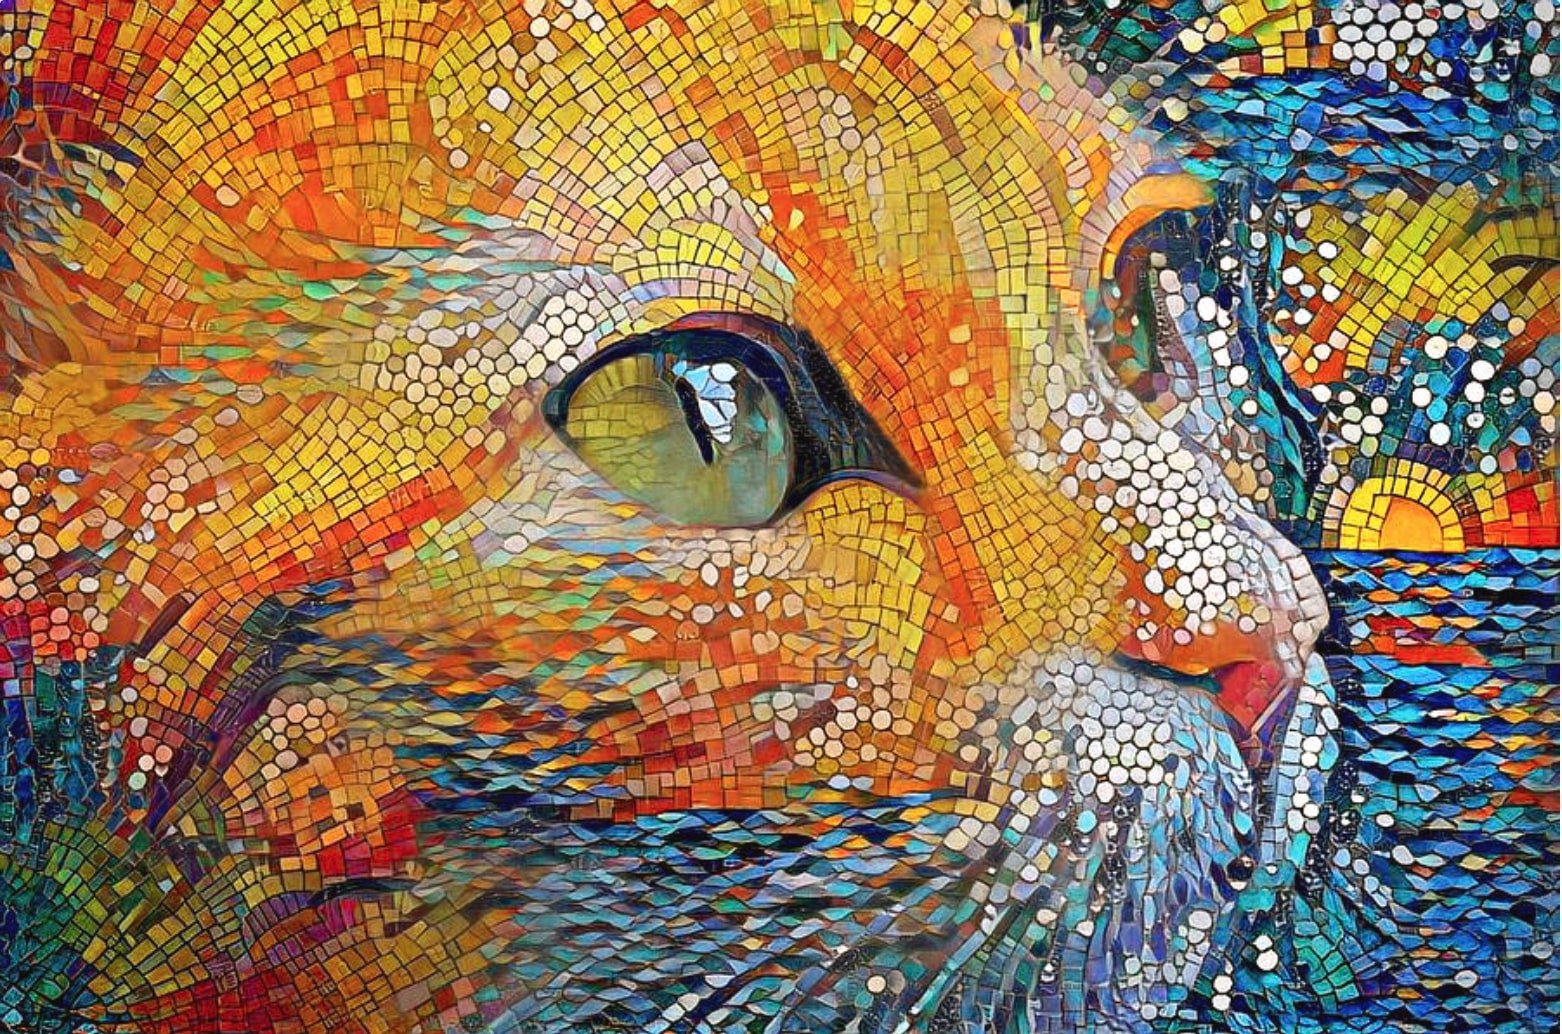
\includegraphics[width=\textwidth]{/Users/Michael/Documents/MDLforBeginners/Chapter3/Code/Images/Mosaic1.jpg}
	\caption{Ginger Cat by Peggy Collins (digital artwork)}
\end{figure}	
\begin{python}
print(im_mosaic1[:10, :10, 1])
# [[246 190 116  51  30  21   0   6  28  42]
#  [188  88  48  52  40  20   4  12  28  39]
#  [108  40  37  55  43  27  17  15  24  35]
#  [ 35  34  41  39  35  32  21  18  21  31]
#  [ 20  24  25  26  34  26  13  23  23  29]
#  [ 35  25  24  29  28  19  17  26  25  29]
#  [ 28  23  24  22  15  17  24  22  23  25]
#  [ 33  29  18  15  18  17  15  12  18  19]
#  [ 18  14  13  16  19  19  19  18  15  11]
#  [  8   6   8  16  23  26  24  21  20  15]]	
\end{python}
\end{example}

\begin{definition}
	我们将多媒体数据集和数据阵组合构成的数据形态成为\textit{数据群}或者\textit{大数据}。数据群或大数据,在业界也被称为\textbf{有标注的数据群}。
\end{definition}

\begin{example}
比如,下面这个数据群,就是一个有标注的数据群。\mn{大数据时代,数据的标注准确度和密集度,成为衡量数据群质量的重要指标。国际上,目前美国的数据群质量最高,其次是英国和德国。中国的数据群目前取胜于量,对于质的追求,还需要一定的时间。}
\begin{table}[H]
	\centering
	\renewcommand{\arraystretch}{1.5}
	\begin{tabular}{ccccc}
	\hline 
		图片(1400, 1400, 3) & 年份 & 地点 & 备注1 & 备注2 \\
		\hline 
		图1 & 2016 & 桥 & 青岛 & 红色 \\
		图2 & 2020 &  伦敦 & 人 & 女 \\
		图3 & 2013 & 成都& 熊猫 & 国宝\\
		\hline 
	\end{tabular}
\end{table}
\end{example}


\subsubsection{损失方程(Loss Function)}

人工智能中很多模型,包括神经网络学习模型都需要有标注的数据群。比如我们通过想要训练神经网络学习模型辨别图片中的人物的性别,那么就需要具有\textit{性别标注}的图片数据群。拥有了标注的数据,就可以训练人工智能模型,从而可以调整模型参数,来提升预测准确度。而用来衡量准确度的方程就需要损失方程。

\begin{definition}
	假设数据群标注过的数据准确可靠,在人工智能模型中,模型在整合输入数据且加工计算后输出的结果与数据群标注的数据差别的方程称为\textit{损失方程(Loss Function)}。
\end{definition}

\begin{example}
比如我们想要通过人工智能来判定图片中人类的性别,下面的表格中给出了最为简单的一种损失方程。
\begin{table}[H]
	\centering
	\renewcommand{\arraystretch}{1.5}
	\begin{tabular}{cccc}
	\hline 
		图片(1400, 1400, 3) & 标注(1-男,0-女) & 模型预测 & 差异\\
		\hline 
		图1 & 1 & 0 & 1 \\
		图2 & 0 & 1 & 1 \\
		图3 & 1 & 1 & 0 \\
		\hline 
	\end{tabular}
\end{table}
用$\hat{Y}$来代表预测的结果,$Y$来代表标注结果,那么损失方程为:
\begin{align*}
	L(Y, \hat{Y}): |Y-\hat{Y}| 
\end{align*}
\end{example}

\begin{remark}
损失方程(Loss function) 有很多设计。设计或者选择损失方程的依据是为了更好得训练人工智能的模型,从而提升预测准确度。后面我们还会逐渐介绍不同的损失方程,但是其一般形式为:
\begin{align*}
	L: (Y, \hat{Y}): \ \to \rn 
\end{align*}	
\end{remark}

\subsubsection{初始数据群处理}

在具体的人工智能实践中,我们很多时间实际上是花在处理初始数据群上的\mn{Data scientists spend 80\% of their time cleaning data rather than creating insights.}。这是因为初始数据群的整洁程度和能否直接被人工智能模型接受,会影响我们后面对模型的训练和各类模型的调试。因为处理初始数据群非常重要,所以很多公司会聘请专门的数据专家进行数据整理和矫正。希望同学们在具体的操作中,也有数据集群意识。因为本章的神经网络模型处理较多的是图片,所以我们接下来重点介绍图片的多媒体数据集合构成。


\subsubsection{向量、矩阵和其相关的运算}

无论是\textit{多媒体数据集}还是\textit{数据阵},除去其标注的信息,具体的数都是储存在矩阵中的。

\begin{definition}
	\textit{矩阵}(Matrix)是一个按照长方阵列排列的复数或实数集合。对一个矩阵的简单描述可以为 $m \times n$ 的矩阵,即该矩阵有$m$ 行,$n$列. $m \times n$也被称为矩阵的大小。
\end{definition}
\begin{example}
比如,我们有$3 \times 3 $的矩阵$A$ 和$2 \times 3$ 的矩阵$B$。
\begin{align*}
	 A = \begin{bmatrix}
	1 & 3 & 4 \\
	2 & 5 & 8 \\
	3 & 9 & 7
\end{bmatrix}, & & B = \begin{bmatrix}
	3.2 & 1.9 & 5.7 \\
	4.1 & 5.8 & 9.3 \\
\end{bmatrix}
\end{align*}	
\end{example}

\begin{definition}
	矩阵中单独的一行被成为\textit{行向量}(row vector), 单独的一列别成为\textit{列向量}(column vector)。
\end{definition}
\begin{example}
比如在上面的矩阵$A$中,	我们有以下单独的向量:
\begin{align*}
	A_{r2} = [2 \ 5 \ 8],  & & A_{c2} = \begin{bmatrix}
		3 \\
		5 \\
		9 
	\end{bmatrix}
\end{align*}
\end{example}

\begin{definition}
	现有同样大小的$m \times n$的矩阵 $A, B$, 我们定义矩阵的加法($+$)运算为:
	\begin{align*}
		A + B = \begin{bmatrix}
			(a_{11} + b_{11}) & (a_{12}+b_{12}) & \cdots & (a_{1n}+b_{1n}) \\
			a_{21} + b_{21} & a_{22}+b_{22} & \cdots & a_{2n}+b_{2n} \\
			\vdots & \ddots & & \vdots \\
			a_{m1} + b_{m1} & a_{m2}+b_{m2} & \cdots & a_{mn}+b_{mn} \\
		\end{bmatrix}
	\end{align*}
	其中,$a_{ij}$ 为矩阵$A$中第$i$行第$j$列元素,$b_{ij}$ 为矩阵$B$中第$i$行第$j$列元素。
\end{definition}

\begin{remark}
矩阵的加法只能在同样大小的矩阵中进行,即同位元素相加。	
\end{remark}

矩阵最早的提出是为了解决多项式的求解,比如下面方程组的转换。
\begin{align*}
	2x_1 + 3x_2 + 7x_3 & = 9 \\
	4x_1 + 5x_2 + 8 x_3 & = 10 \\
\end{align*}
可以用矩阵的乘法来表示:
\begin{align*}
	\begin{bmatrix}
		2 & 3 & 7 \\
		4 & 5 & 8 
	\end{bmatrix} \begin{bmatrix}
		x_1 \\
		x_2 \\
		x_3 
	\end{bmatrix} = \begin{bmatrix}
		 9 \\
		 10 
	\end{bmatrix}
\end{align*}

\begin{definition}
	现有$m \times n$ 的矩阵A 和 $n \times k$的矩阵$B$, 我们定义矩阵的乘法$\cdot$为
	\begin{align*}
		(A \cdot B)_{ij} = \sum_{r=1}^n a_{ir}b_{rj} = a_{i1}b_{1j} + a_{i2}b_{2j} + \cdots + a_{in}b_{nj}
	\end{align*}
	其中$(A \dot B)_{ij}$是两个矩阵相乘后的第i行第j列元素。
\end{definition}

\begin{remark}
取任意$a \times b$ 矩阵A 和$c \times d$ 矩阵 B, 如果$b \neq c$,则两个矩阵不可以相乘。	
\end{remark}

\begin{example}
计算下列矩阵的乘法
\begin{align*}
	\begin{bmatrix}
		2 & 3 & 7 \\
		4 & 5 & 8 
	\end{bmatrix} \begin{bmatrix}
		1 \\
		0 \\
		-1 
	\end{bmatrix} = \ ? & & \begin{bmatrix}
		1 & 3 & 3 \\
		2 & 8 & 4 \\
		3 & 9 & 1 
	\end{bmatrix} \begin{bmatrix}
		3 & 2 \\
		1 & 0 \\
		-1 & 8 
	\end{bmatrix} = \ ?
\end{align*}	
\end{example}

\subsubsection{卷积运算(Convolution)}

卷积运算(Convolution)是图形处理中特有的一种运算方式。其目的是\textbf{系统性一次性得}对原始图片进行快速处理。我们之前已经讲解过图形的储存形式,而且在课前预习中的习题中也特别对卷积运算进行了铺垫,接下来我们就更加规范得对这个概念进行学习。

\begin{definition}
	给定一个长度为$m$的向量$A$和一个长度为$n$的向量$B$, 其中$n > m$:
	\begin{align*}
		A & = [a_1, a_2, \cdots, a_m ] \\
		B & = [b_1, b_2, \cdots, \cdots, a_n]
	\end{align*}
	我们称$A$为\textit{参数(核)向量}\mn{kernel vector},$B$为\textit{数据向量},其卷积运算(convolution)$*$定义为
	
	\begin{algorithm}[H]
	\SetAlgoLined
	\caption{Convolution Operation}
	初始化长度为$n-m+1$的向量$C = [c_1, c_2, \cdots, c_{n-m+1}]$ \;
	$C = A * B $ \; 其中,每一个元素的计算方法为\;
	\For {$i \ in \ [1:n-m+1]$}{$c_i = \sum_{k=1}^m a_k b_{k+i-1} = a_1 b_i +  a_2 b_{i+1} +\cdots + a_m b_{i+m-1}$}
	\end{algorithm}
\end{definition}

\begin{example}
	现有参数向量$A=[1, 3, 4]$ 和数据向量$B = [5, 6, 7 , 8 , 9]$,那么
	\begin{align*}
		A * B & = [34, 40, 46]\\
		34 & = 1\times 5 + 3 \times 6 + 4 \times 7 \\
		40 & = 1 \times 6 + 3 \times 7 + 4 \times 8 
	\end{align*}
\end{example}

\begin{definition}
	给定一个$m \times n$的矩阵$A$,和一个$k \times l$的矩阵$B$,并且$k > m, l > n$, 那么矩阵$A$被叫作\textit{参数(核)矩阵}\mn{kernel matrix},矩阵$B$被称为\textit{数据矩阵}。那么矩阵$A$和$B$的卷积运算定义为
	\begin{align*}
		A * B = \text{移动参数向量对数据向量进行对位求积后求和}
	\end{align*}
	运算过程如下图所示(来源:Irhum Shafkat, 2018)\mn{矩阵的卷积有很多种,更多的介绍请参考该网站:\url{https://towardsdatascience.com/intuitively-understanding-convolutions-for-deep-learning-1f6f42faee1}}。
\end{definition}

\begin{figure}[H]
	\centering
	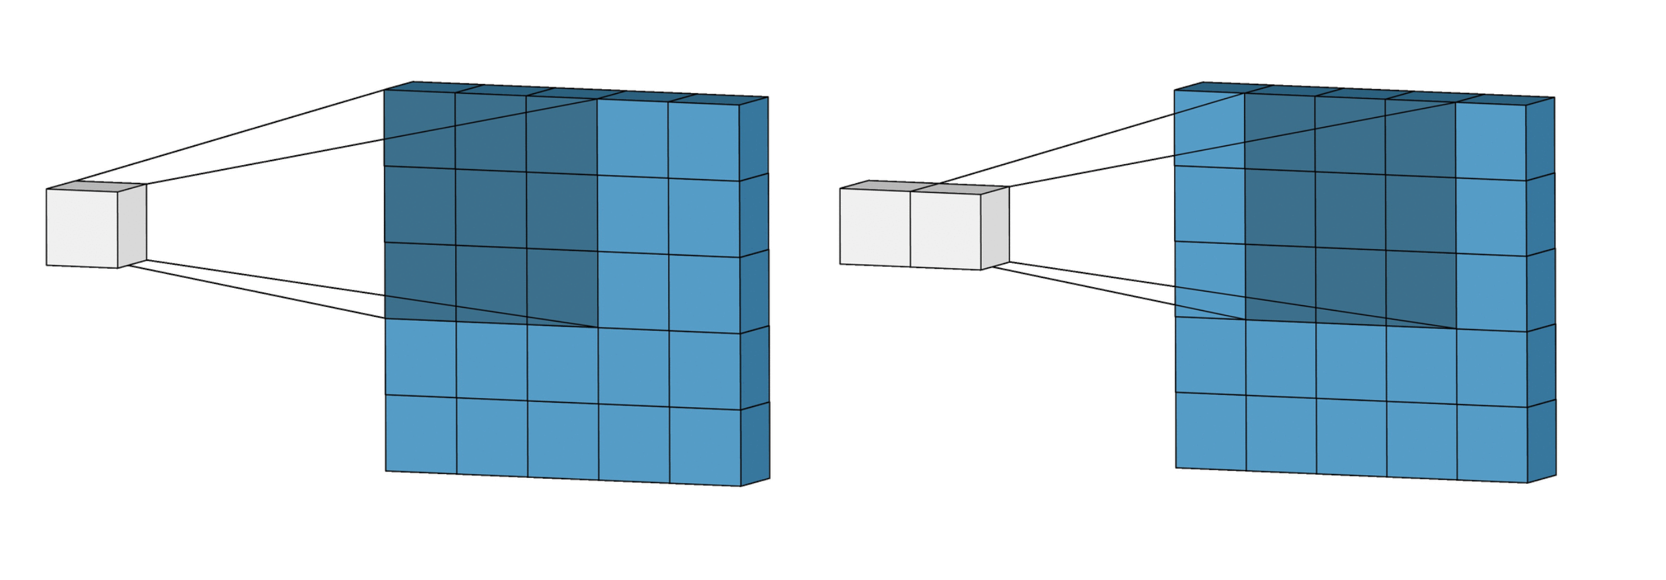
\includegraphics[width=\textwidth]{fig/mtconvo}
	\caption{基本矩阵卷积计算}
\end{figure}

\begin{remark}
	矩阵的卷积运算目的是想要通过参数矩阵来对数据矩阵进行进一步的处理。之所以需要这个处理过程是因为
	\begin{itemize}
		\item 原始多媒体数据集维数较大,比如图3.4中的猫有$(1400, 1400, 3)$,即$1400 \times 1400 \times 3 = 588000$个数(元素)组成。通过卷积运算后数据集的维数会有所下降,从而节省模型训练时间;
		\item 原始多媒体数据集的特征不明显,需要通过参数矩阵的卷积运算后来进行优化;
		\item 卷积在图像识别中的应用原因还有其它的,以后我们会结合具体案例进一步讲解。\mn{卷积运算主要应用在图像识别中,在其它领域,比如金融数据的人工智能模型,则没有被那么广泛得使用。}
	\end{itemize}
\end{remark}

\begin{example}
我们手动计算一种标准的卷积形式,给定参数核矩阵$A$和数据矩阵$B$为
\begin{align*}
	A = \begin{bmatrix}
		1 & -1 \\
		1 & 2 
	\end{bmatrix} & & B= \begin{bmatrix}
		1 & 2 & 1 \\
		2 & 3 & 6 \\
		0 & 5 & 7 
	\end{bmatrix}
\end{align*}	
我们演示计算结果矩阵($C = A*B$)的第一个元素\mn{$C=A*B$的最终结果为\begin{align*}
	C = \begin{bmatrix}
		7 & 16 \\
		9 & 16
	\end{bmatrix}
\end{align*} 你会发现$C$中元素最大值是$14$,刚好在$B$的右下角,这是巧合吗?(显示不是,否则我也不发发问了)}
\begin{align*}
	C_{11} = 1\times 1 + (-1) \times 2 + 1 \times 2 + 2 \times 3 = 7 
\end{align*}
\end{example}


\begin{example}
为帮助同学们理解参数卷积的重要性,我们特别详细分析一个生活常见的具体案例。下面的表格是一个班级内几名同学的不同学科的成绩表,我们来计算不同的参数卷积矩阵可以给出不同的`评估'结果(这个评估结果可以理解成我们机器学习的一个运算结果)。
\begin{figure}[H]
	\centering
	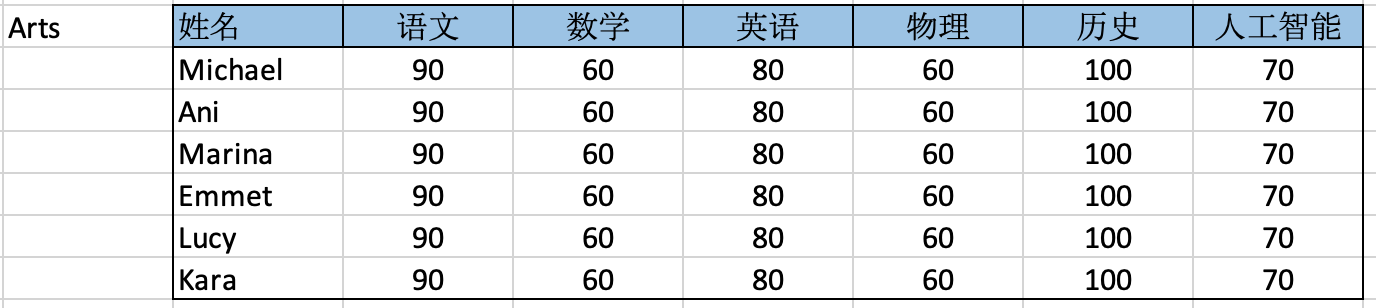
\includegraphics[width=\textwidth]{fig/artsgrade}
	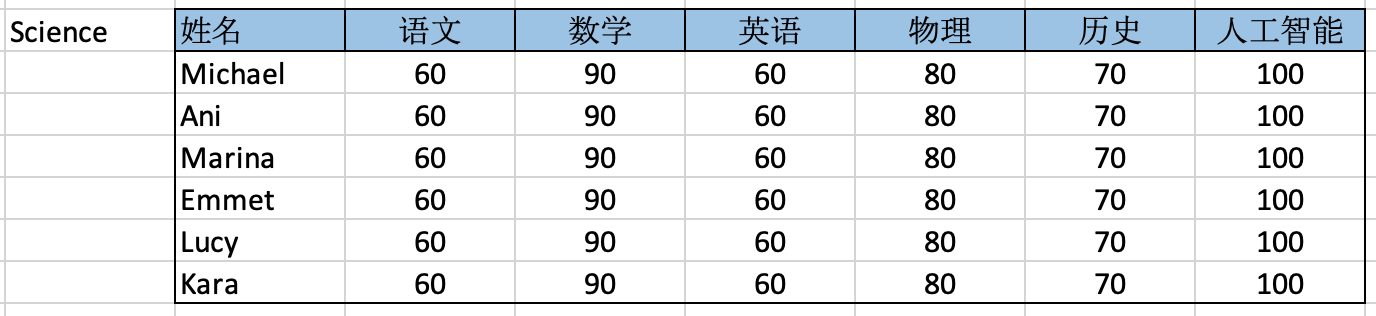
\includegraphics[width=\textwidth]{fig/sciencegrade}
\end{figure}
其中参数核(kernel)矩阵给定为
\begin{align*}
	K = \begin{bmatrix}
		1 & 0 & $-$1$$ \\
		1 & 0 & $-$1$$  \\
		1 & 0 & $-$1$$  
	\end{bmatrix}
\end{align*}
将文科生(arts)和理科生(science)的数据阵进行两次卷积运算:
\begin{align*}
	A \Rightarrow \begin{bmatrix}
		30 &    0  &   -60  &    -30 \\
       30  &     0  &    -60  &    -30   \\        
       30  &     0  &    -60  &   -30 \\
       30  &    0  &    -60  &   -30 
	\end{bmatrix} \Rightarrow \begin{bmatrix}
		270 & 90 \\
		270 & 90 
	\end{bmatrix} & & 	S \Rightarrow \begin{bmatrix}
	   0 & 30 & -30 & -60 \\
       0 & 30 &  -30 & -60 \\
        0 & 30 &  -30 & -60 \\
       0 & 30 &  -30 &  -60
	\end{bmatrix} \Rightarrow \begin{bmatrix}
		90 & 270 \\
		90 & 270 
	\end{bmatrix}
\end{align*}
两个矩阵看起来很相似,只是列向量顺序不同。如果我们将两个矩阵按照此前的顺序进行标注,可以得出下面的表格:\mn{如果你没有觉得数学像变魔术一样把复杂问题简单化的话,我也只能表示要喝一瓶王老吉了。}
\begin{table}[H]
\renewcommand{\arraystretch}{1.2}
	\centering
	\begin{tabular}{|l|cc|}
	\hline 
		学科/成绩集成 & 文科生(arts) & 理科生(science) \\
		\hline 
		文& 270 & 90 \\
		科& 270 & 90 \\
		\hline 
		理& 90 & 270 \\
		科& 90 & 270 \\
		\hline 
	\end{tabular}
\end{table}
\end{example}

复杂神经学习模型要比以上的例子复杂的多,但是基本流程却非常相似,具体的计算和演化逻辑也可以说`如出一辙'。我们可以把神经网络深度学习的模型再一次概况为:\textbf{通过对输入端的数据群(大数据)进行标注和整理后,建立一个人工智能构架,并设定目标函数(损失方程),对所建立的构建(或模型)进行反复训练,直到找到符合我们目标函数要求的参数核矩阵。}

\noindent
下面是本讲内容使用的Python程序,有兴趣的同学可以自己复制后运行和进行改进调试。
\begin{python}
# Chapter 3 Lecture 1
# 课堂讲义
# @ Michael

# Import essential packages
# 导入必要扩展

import numpy as np
from scipy import signal

# vector convolution 向量卷积
a = np.array([1, 2, 3])
b = np.array([5, 6, 7, 8, 9])
np.convolve(a, b, 'valid')  # array([34, 40, 46])

# matrix convolution example 1
kernela = np.array([[1, -1], [1, 2]])
datamatrix = np.array([[1, 2, 1], [2, 3, 6], [0, 5, 7]])
print(signal.convolve2d(kernela, datamatrix, 'valid'))
# 注意该方程中的卷积方式,与我们定义的有所不同


def matrixConv(kenl, dtm):
    # Assume size of kenel is less than datamatrix
    # 假设参数核矩阵小于数据矩阵
    m = np.shape(kenl)[0]
    n = np.shape(kenl)[1]
    k = np.shape(dtm)[0]
    l = np.shape(dtm)[1]
    resltmtx = np.zeros([k-m+1, l-n+1])
    for i in range(resltmtx.shape[0]):
        for j in range(resltmtx.shape[1]):
            temp = 0
            for u in range(m):
                for p in range(n):
                    temp += kenl[u, p] * dtm[u+i, p+j]
                    resltmtx[i, j] = temp
    return(resltmtx)


# test the function
matrixConv(kernela, datamatrix)


# matrix convolution example 2
grade_arts = np.ones([6, 6])
grade_science = np.ones([6, 6])
grade_dist1 = [90, 60, 80, 60, 100, 70]
grade_dist2 = [60, 90, 60, 80, 70, 100]
for i in range(len(grade_dist1)):
    grade_arts[:, i] = grade_arts[:, i] * grade_dist1[i]
for j in range(len(grade_dist2)):
    grade_science[:, j] = grade_science[:, j] * grade_dist2[j]

print(grade_arts)
print(grade_science)

kernel_para = np.array([[1, 0, -1], [1, 0, -1], [1, 0, -1]])
conv_arts = signal.convolve2d(grade_arts, kernel_para, 'valid')
# array([[-30.,   0.,  60.,  30.],
#        [-30.,   0.,  60.,  30.],
#        [-30.,   0.,  60.,  30.],
#        [-30.,   0.,  60.,  30.]])
signal.convolve2d(conv_arts, kernel_para, 'valid')
# array([[270.,  90.],
#        [270.,  90.]])

# use self-wrote function
conv_arts2 = matrixConv(kernel_para, grade_arts)
# array([[ 30.,   0., -60., -30.],
#        [ 30.,   0., -60., -30.],
#        [ 30.,   0., -60., -30.],
#        [ 30.,   0., -60., -30.]])
matrixConv(kernel_para, conv_arts2)
# array([[270.,  90.],
#        [270.,  90.]])


conv_science = signal.convolve2d(grade_science, kernel_para, 'valid')
conv_science.shape
# array([[  0., -30.,  30.,  60.],
#        [  0., -30.,  30.,  60.],
#        [  0., -30.,  30.,  60.],
#        [  0., -30.,  30.,  60.]])
signal.convolve2d(conv_science, kernel_para, 'valid')
# array([[ 90., 270.],
#        [ 90., 270.]])

#use self-wrote function
conv_science2 = matrixConv(kernel_para, grade_science)
# array([[  0.,  30., -30., -60.],
#        [  0.,  30., -30., -60.],
#        [  0.,  30., -30., -60.],
#        [  0.,  30., -30., -60.]])
matrixConv(kernel_para, conv_science2)
# array([[ 90., 270.],
#        [ 90., 270.]])
\end{python}


Bonjour,我们这一节的课堂讲义就到此结束了,下面你要进行课后练习了。这些课后练习并不复杂,只是需要你动脑+动手。

\hfil

\noindent
\textcolor{purple}{疑难解答}:如果有相关疑问,请扫描下面的二维码,讲你的问题输入,老师会尽快答疑解惑:$\heartsuit$。 \begin{marginfigure}
	\centering
	
\includegraphics[width=\textwidth]{fig/C3C2qrcode}
\end{marginfigure}


\newpage
\subsection{课后练习C3}

\begin{fullmodel}
\begin{question}{思考题C3-Q1}
	Michael是一名研修植物学的大学生,他一直梦想只用通过手机拍照后,计算机就可以自动配图和文字,对他所拍的植物进行一份文档生成,而不是他亲自去采集植物,阅读资料,并且撰写有关植物学的报告。解决该类问题除了图像处理之外,还需要自然语言的处理。你认为他的梦想会在未来会实现吗?实际上,Michael爱好诗歌,他喜欢写短行诗后配上图片发到朋友圈上,下面是他发的一条朋友圈。请问你可以训练计算机写诗吗?
	\begin{figure}[H]
		\centering
		\begin{subfigure}[b]{0.45\textwidth}
			\centering
			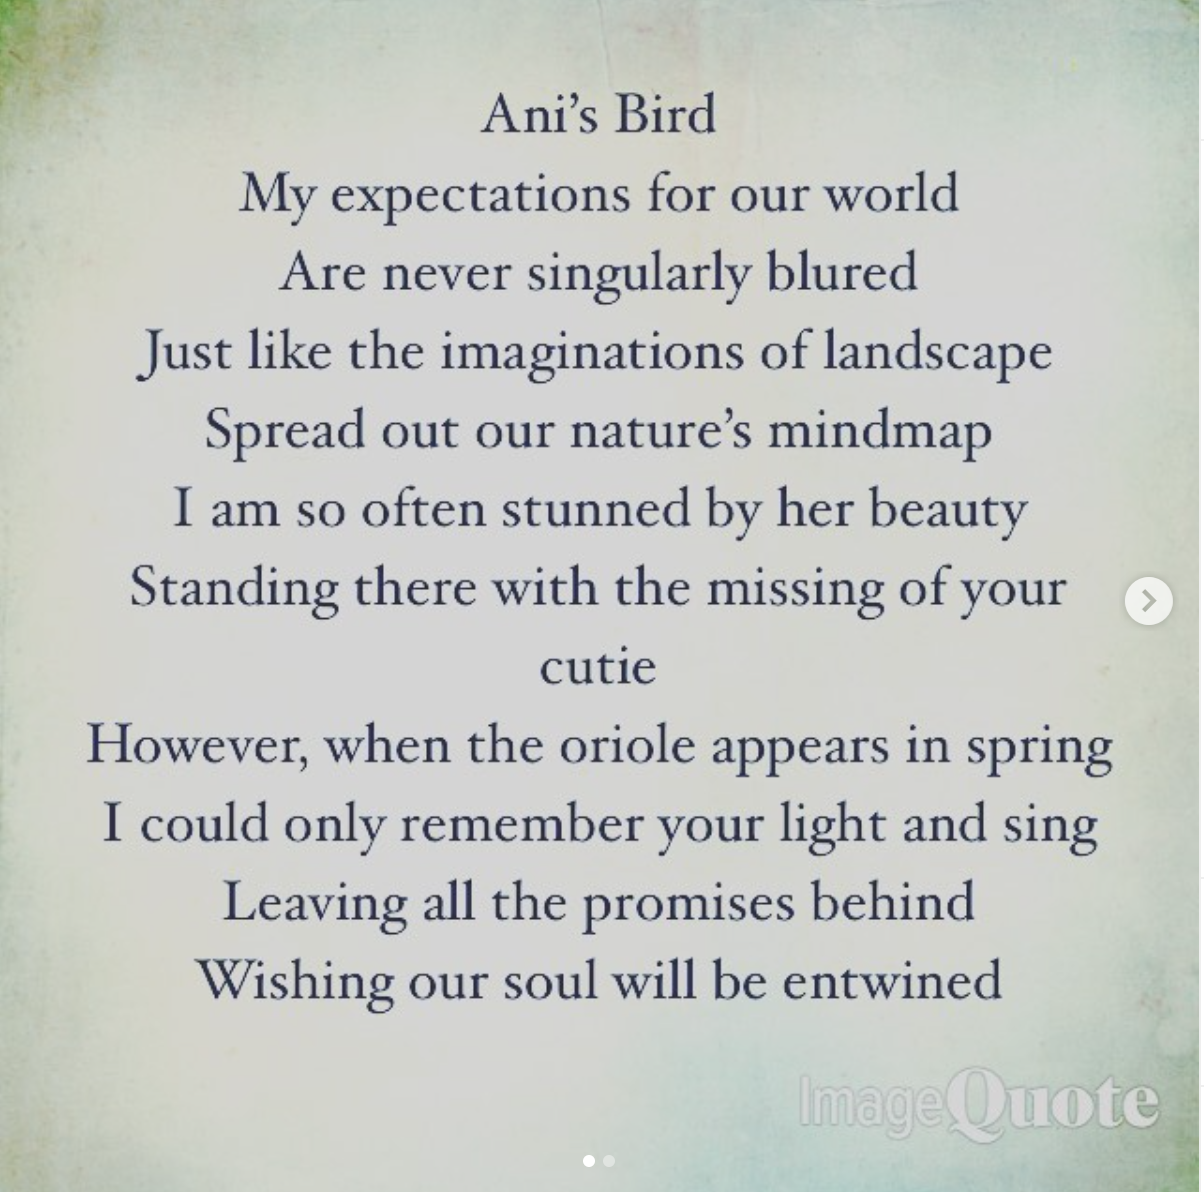
\includegraphics[width=\textwidth]{fig/poetry1}
		\end{subfigure}
		\begin{subfigure}[b]{0.45\textwidth}
			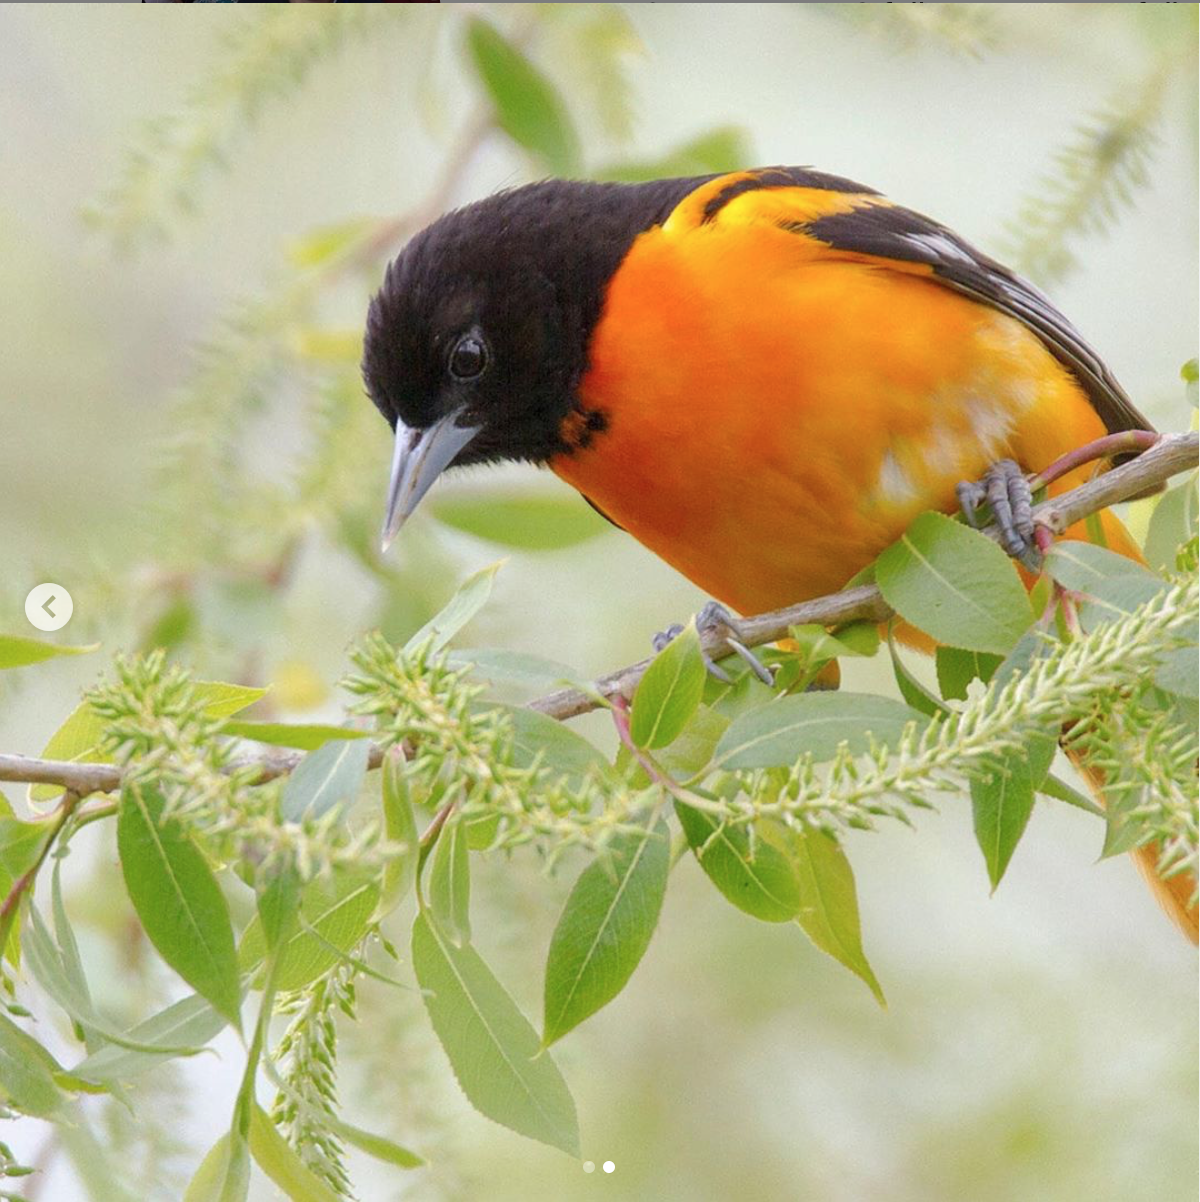
\includegraphics[width=0.99\textwidth]{fig/peotry2}
		\end{subfigure}
	\end{figure}
\end{question}	
\end{fullmodel}


\begin{fullmodel}
\begin{question}{设计题 C3-Q2}
	下面的表格中有九个描述,根据这九个描述,将你的数据构成一个$9 \times 9$的矩阵。然而设计一个损失方程(Loss function),然后计算你跟班里的同学谁最\textit{相像}。其中性别代码1指男性,0指女性。所有的数据均采用公有制单位,比如身高176cm,在矩阵中填176即可,视力1.5等
	\begin{figure}[H]
		\centering
		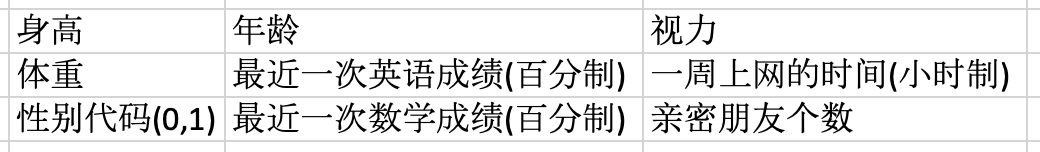
\includegraphics[width=0.7\textwidth]{fig/c3q2}
	\end{figure}
\end{question}
\noindent
提示:损失方程最简单就是,将矩阵的每个元素相减,然后求和。当然你也可以根据自己的喜好,对每个描述进行有比重的衡量。	根据你设计的损失方程,使用Python计算你与其它至少一位同学的相像值。
\end{fullmodel}


\begin{question}{作图题 C3-Q3}
	该题目具有承上启下的作用,虽然很简单,但是所蕴含的道理`法力无边'。给定方程$f(x) = -x^2+ 6x-2$, 下面是其图像,在这个图像中$x=2, x = 4, x =5$三个点上,画三条切线\mn{英文好的同学,可以阅读老师编写针对该问题的深入解释:\url{https://github.com/Michael-yunfei/MachineLearning/blob/master/GraidentDescent/Gradient.pdf}}。
	\begin{figure}[H]
		\centering
		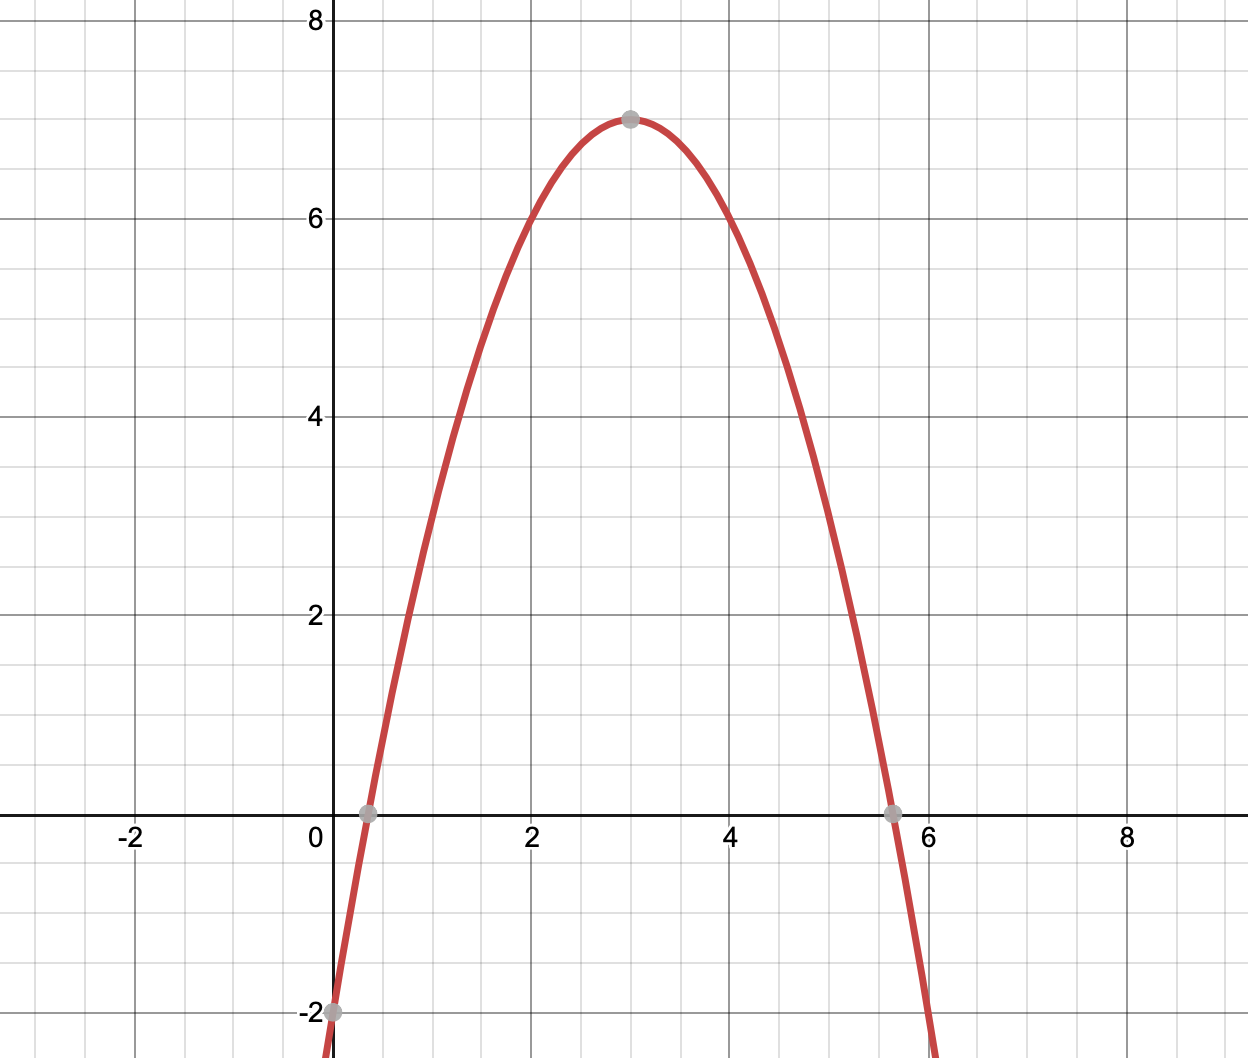
\includegraphics[width=0.6\textwidth]{fig/c3q3}
	\end{figure}
\end{question}


\begin{question}{计算题 C3-Q4}
	完成下列矩阵计算,请先手动计算,然后用Python计算。给定矩阵
	\begin{align*}
		A = \begin{bmatrix}
			3.2 & 1.7 \\
			5.1 & 8.9 
		\end{bmatrix}; \ \ \ B = \begin{bmatrix}
			0.9 & -1 \\
			 -1 & 0.1 
		\end{bmatrix}; \ \ \ C = \begin{bmatrix}
			2 & 3 & 9 \\
			7 & 8 & 6 \\
			1 & 0 & 5 
		\end{bmatrix}
	\end{align*}
	求矩阵的加法和卷积如下
	\begin{align*}
		A + B & = \ \ ? \\
		B * C &= \ \ ? \\
		B * A & = 
	\end{align*}
\end{question}


\noindent
khorosho(俄语,很好)!下节见。

























\end{document}
